\documentclass[../main.tex]{subfiles}

\begin{document}
	\section{Turning Effect of Forces}
	\begin{preamb}
		Objects do not only move in a straight line, they can also move in curves and circles and all kinds of funny shapes. In this chapter we will explore how we can make an object turn by applying a force.
	\end{preamb}

	\subsection{Moment}
		\pdef{Moment}{A moment is the \textbf{turning effect} of a force \textbf{around a pivot}. It is equal to the numerical product of the force applied \(F\) and the perpendicular distance \(r\) from the pivot \[M_O = r \times F\] The SI unit of moment is newton metre [\si{\newton \metre}].}
		
		\begin{center}
			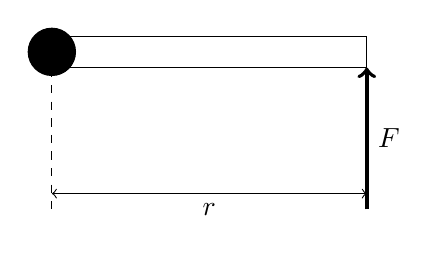
\begin{tikzpicture}
				\filldraw [fill=black] (0,0) circle (3mm);
				\draw (0,-0.2) rectangle (4,0.2);
				\draw [line width=0.5mm, ->] (4,-2) -- (4,-0.2) node[pos=0.5, anchor=west] {\(F\)};
				\draw [dashed] (0,0) -- (0,-2);
				\draw [<->] (0,-1.8) -- (4,-1.8) node[pos=0.5, anchor=north] {\(r\)};
			\end{tikzpicture}
		\end{center}
	
		\pdef{Rotational Equilibrium}{An object is said to be in rotational equilibrium if the sum of \textbf{anticlockwise moments} about a pivot point is \textbf{equal} to the sum of \textbf{clockwise moments} around the same pivot point.}
		
	\subsection{Centre of Gravity}
		\pdef{Centre of Gravity}{The centre of gravity, or centre of mass, is a point where the weight of an object seems to be acting on. The centre of gravity can lie outside an object.}
		
	\subsection{Stability}
		An object can be in stable, unstable, or neutral equilibrium.
		\begin{center}
		\begin{tabularx}{\linewidth}{X|XXX}
			\hline \hline
			Type of equilibrium & Stable & Unstable & Neutral \\
			\hline
			Centre of gravity & Low & High & \\
			Base area & Large & Narrow & A line of contact points with surface \\
			Slight displacement & Return to equilibrium & Topple over & Stay in new position \\
			\hline \hline
		\end{tabularx}
		\end{center}
	
		An object's stability can be increased by lowering the height of the centre of gravity, or increasing the base area of the object.
\end{document}